
\subsection{Sensordaten-Fusion}
\label{headtracking_fusion_subsec}
Die Sensordaten-Fusion beschreibt die Verknüpfung von mehreren Sensoren um Informationen besserer Qualität zu gewinnen. In diesem Projekt gilt des die aufbereiteten Daten aus beiden Gyroskopen, Beschleunigungsensor und Magenetometer derart zu fusionieren, dass letztlich die zu ermittelnde \emph{Orientierung} des Kopfes möglichst exakt bestimmt werden kann. Da die bereits vorgestellten Sensoren jeweils eigene Vor- und Nachteile hat müssen diese bestmöglich ausgenutzt werden. In den folgenden Abschnitten werden unterschiedliche Fusionsansätze dargestellt und entsprechend der Aufgabenstellung des Projekts bewertet. 

\subsubsection{Madgwick-Filter}
Die Filterung nach Madgwick \cite{madgwick2010efficient} gilt als neuartiger Ansatz zur Bestimmung der Orientierung basierend auf Gyroskop, Beschleunigungssensor und Magnetometer.
Es wird dabei versucht die magnetische Distorsion sowie der Bias-Trift des Gyroskopes auszugleichen.
Berechnungsgrundlage ist dafür eine auf Quaternionen-basierte Darstellungsform, welche in einem Gradienten-Abstiegsverfahren zum Einsatz kommt.
Vorteile dieses Ansatzes sind seine niedrigen Berechnungskosten, Effektivität bei niedrigen Sampleraten und ein hoher Grad an Parametrisierung der eine Anpassung an die jeweiligen Sensor- und Umgebungscharakteristiken zulässt.

Auch wenn der Madgwick-Filter bereits als fertige ROS-Node\footnote{\url{http://wiki.ros.org/imu_filter_madgwick}} vorhanden ist und bessere Ergebnisse als der Kalman-Filter liefern soll, haben wir uns gegen den Madgwick-Filter entschieden, da unsere bestehende Implementierung nur schwer an den Madgwick-Filter angepasst werden konnte und dadurch der erzielte Mehrwert so nur schwer nachvollziehbar bzw. debuggbar gewesen ist. 


\subsubsection{Kalman-Filter}
Beim Kalman-Filter Verfahren \todo{cite} handelt es sich um eine probabilitische Methode der Zustandsschätzung.
Dabei fließen in einem ersten \emph{Prädiktionsschritt} vorhergemachte Annahmen inklusive dazugehöriger Fehlerwahrscheinlichkeiten in die Berechnung ein.
Danach wird in einem zweiten Schritt, der \emph{Innovationsschritt}, eine Beobachtung mit dazugehöriger Messungenauigkeit mit einbezogen.

Um bei einer fehlerbehafteten Beobachtung den Systemzustand zu korrigieren, müssen diese Beobachtungen über mathematische Gleichungen beschreibbar und Fehlerverteilungen für Sensoren bekannt sein. Diese Informationen sind uns während der Bearbeitung des Projekts nicht bekannt gewesen.
Infolgedessen konnte eine Modellierung gemäß dem Kalman-Filters nicht durchgeführt werden. 
Des weiteren war unklar ob durch eine solche Umsetzung tatsächliche Vorteile erzielt werden können, da die Änderung eines plötzlichen Ereignis (Kurvenfahrt) über mehre Zeitschritte hinweg angepasst wird und somit eine mögliche Latenz hinzugefügt werden könnte.

\subsubsection{Komplementär-Filter}
Nach Brooks und Iyengar \cite{Brooks.1998} hat eine komplementäre Fusion das Ziel, die Genauigkeit von Daten zu verbessern. 
Dabei wirken die Sensoren unabhängig voneinander und liefern unterschiedliche Erkenntnisse und Sichtbereiche, die die Orientierung zu unterschiedlichen Zeiten verbessert.

Die Gyroskope sind wie bereits erwähnt bei einer langen Laufzeiten fehleranfällig und erzeugen einen Drift. 
Daher wird im ersten Schritt eine SLERP-Interpolation (Sperical Linear Interpolation) eingesetzt, die bei jedem Zeitschritt die Orientierung der Gyroskope zu $95\%$ und Orientierung des Beschleunigungssensor zu $5\%$ berücksichtigt. Hierbei wird das \emph{roll} und \emph{pitch} gestützt. Der zweite Schritt zielt auf die Verbesserung von \emph{yaw} ab. Eine weitere Interpolation verrechnet dieses Ergebnis mit den aufbereiteten Magnetometerwerten zu $5\%$ pro Zeitschritt. Formal lässt sich die Gewichtung folgendermaßen beschreiben:

\begin{align}
F_P &= \textbf{\textit{Gyro}}*~0.95~~+~~\textbf{\textit{Acc}}~~*~0.05\\
\notag\\
F_G &= ~F_P~~*~0.95~~+~~\textbf{\textit{Mag}}~*~0.05
\end{align}

%\begin{equation}
%	F_G = F_P~*~0.95~+~\textbf{\textit{Mag}}~*~0.05
%\end{equation}

Eine Übersicht der Fusionierung mit dem Komplementär-Filter ist Abbildung \ref{fig:fusion_complementary} zu entnehmen.

\begin{figure}[ht]
	\begin{center}
		\scalebox{0.77}{
	\begin{tikzpicture}[%
		>=stealth, % Aussehen der Pfeilspitzen
		->, % Linien als Verbindungslinien
		looseness=.7, % Kr"ummung der Pfeile mit Option ’bent’
		auto, % Position des Ankers f"ur Node Labels
		color=black, % Farbe aller Linien
		%text=red, % Textfarbe in den Matrix-Nodes
		line width=1pt, % Linienst"arke f"ur alle Elemente
		text centered
	]
		\tikzstyle{every node}=[shape=rectangle,draw,fill=white,
		anchor=center] % Stil der Node-Beschriftung der
	\node[rectangle, rotate=-30, draw=orange, text width=2.5cm, outer sep=3pt, minimum size=1.5cm] at (0.6,4.5) {\textbf{$\alpha X+(1-\alpha)Y$}};
	\node[rectangle, font=\bfseries, double=green, text width=2.0cm, outer sep=3pt, minimum size=1.5cm](gyro) at (-7.0,5.5) {Gyro};
	\node[rectangle, font=\bfseries, double=green, text width=2.0cm, outer sep=3pt, minimum size=1.5cm](acc) at (-3.0,5.5) {Acc};
	
	\node[rectangle, font=\small, text width=2.5cm, outer sep=3pt, minimum size=1.5cm](interpol1) at (-3.0,2.5) {Interpolation \\ \textit{(SLERP)}};
	
	\node[rectangle, font=\small, text width=2.5cm, outer sep=3pt, minimum size=1.5cm](interpol2) at (-3.0,-2.5) {Interpolation \\ \textit{(SLERP)}};
	\node[rectangle, font=\bfseries, double=green, text width=2.0cm, outer sep=3pt, minimum size=1.5cm](mag) at (-7.0,-2.5) {Mag};
	
	\node[draw=none] at (-0.5, 0.5)(imageAbove) {\scalebox{0.33}{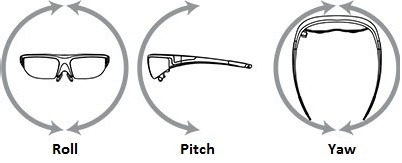
\includegraphics{rpy}}};
	\node[draw=none] at (-1.7, -0.5) {\scalebox{0.02}{
\includegraphics{Yes}}};
	\node[draw=none] at (-0.5, -0.5) {\scalebox{0.02}{
\includegraphics{Yes}}};
	\node[draw=none] at (0.75, -0.5) {\scalebox{0.02}{
\includegraphics{cross}}};
	
	\node[draw=none] at (1.0, -2.5)(imageBelow) {\scalebox{0.33}{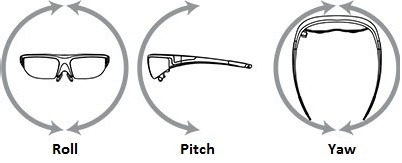
\includegraphics{rpy}}};
	\node[draw=none] at (-0.2, -3.5) {\scalebox{0.02}{
\includegraphics{Yes}}};
	\node[draw=none] at (1., -3.5) {\scalebox{0.02}{
\includegraphics{Yes}}};
	\node[draw=none] at (2.2, -3.5) {\scalebox{0.02}{
\includegraphics{Yes}}};

	\draw[orange, line width=2] (gyro) to[out=-90,in=-180] node[black, above, draw=none, fill=white, font=\small]{$0.95$} (interpol1);
	\draw[orange, line width=2] (acc) -- node[black, above, draw=none, fill=white, font=\small]{$0.05$} (interpol1);
	\draw[orange, line width=2] (interpol1) -- node[black, above, draw=none, fill=white, font=\small]{$0.95$} (interpol2);
	\draw[orange, line width=2] (mag) -- node[black, above, draw=none, fill=white, font=\small]{$0.05$} (interpol2);
	\draw[orange, line width=2] (interpol2) -- (imageBelow);
	
	\end{tikzpicture}}
	\end{center}
   \caption[]{Fusion -- Komplementärfilter}
   \label{fig:fusion_complementary}
\end{figure}